\documentclass[xcolor=dvipsnames]{beamer}
\usetheme{CambridgeUS}
\usepackage[labelformat=simple,
labelsep=period,
font={footnotesize},     %scriptsize, footnotesize, small, normalsize
labelfont=bf,
width=0.9\textwidth,
justification=justified,
singlelinecheck=false
]{caption}
\usepackage[utf8]{inputenc}
\usepackage[spanish, es-tabla]{babel}
\usepackage{amsmath}
\usepackage{subfigure}
\usepackage{amsfonts}
\usepackage{amssymb}
\usepackage{qtree}
\usepackage{tikz}
\usetikzlibrary{calc}
\usepackage{pgfplots,pgfplotstable}
\usepgfplotslibrary{statistics}
\usepackage[T1]{fontenc}
\usepackage{bera}
\usepackage{multirow}
\usepackage{pstricks-add}
\usepackage[capposition=top]{floatrow}
\usepackage{graphicx}
 \usepackage{ragged2e}
 \usepackage{float}
 \usepackage[labelformat=simple,
 labelsep=period,
 font={footnotesize},     %scriptsize, footnotesize, small, normalsize
 labelfont=bf,
 width=0.9\textwidth,
 justification=justified,
 singlelinecheck=false
 ]{caption}
 \usepackage[justification=centering]{caption}
\setbeamersize{text margin left=5pt,text margin right=25pt}
\captionsetup[figure]{labelfont={color=Brown}}
\captionsetup[table]{labelfont={color=Brown}}

\pgfplotsset{compat=1.7}

%%%%%%%%%%%%%%%%%%%%%%%%%%%%%%%%%%%%%%%%%%%%%%%%%%%%%%%%
%%% PAra el diagrama de la diapostiva 10
\usepackage{smartdiagram}
\usetikzlibrary{shapes.geometric} % required in the preamble
\smartdiagramset{
	module minimum width=3cm,
	module minimum height=1cm,
	text width=4.5cm,
	circular distance=3cm,
}
%%%%%%%%%%%%%%%%%%%%%%%%%%%%%%%%%%%%%%%%%%%%%%%%%%%%%%%%%%%
\def\angle{0}
\def\radius{2}
\def\cyclelist{{"orange","blue","red","green"}}
\newcount\cyclecount \cyclecount=-1
\newcount\ind \ind=-1	


\newcounter{saveenumi}
\newcommand{\seti}{\setcounter{saveenumi}{\value{enumi}}}
\newcommand{\conti}{\setcounter{enumi}{\value{saveenumi}}}

\resetcounteronoverlays{saveenumi}
	\tikzset{mynode/.style={inner sep=2pt,fill,outer sep=0,circle}}
	
\author[Carlos Cardona]{Carlos Cardona}
\title{Análisis Cuantitativo I}
\subtitle{Medidas de Dispersión}
\institute[URosario]{Universidad del Rosario}
\date{10 de febrero de 2017}
\begin{document}
	\pgfmathdeclarefunction{gauss}{2}{\pgfmathparse{1/(#2*sqrt(2*pi))*exp(-((x-#1)^2)/(2*#2^2))}%
	}
\maketitle

%%%%%%%%%%%%%%%%%%%%%%%%%%%
\section{Medidas de dispersión}
\begin{frame}{Quiz}
\begin{enumerate}
\item Hallar la media, mediana y moda de la siguiente tabla de distribución de frecuencias: 
\begin{center}
	\begin{table}[H]
		\begin{tabular}{cc} \hline
			X & f \\ \hline
			8&4 \\
			6&5 \\
			4&7 \\
			2&3 \\ \hline
		\end{tabular}
	\end{table}
\end{center}
\item ¿Cuáles son las dos características de un diseño experimental?
\end{enumerate}
\end{frame}
\begin{frame}{Variabilidad}
\begin{itemize}
\justifying
\item Una distribución es descrita por su forma, su tendencia central y su dispersión.
\item La dispersión mide las diferencias entre los valores en una distribución.
\item Una buena medida de dispersión cumple dos objetivos:
\begin{enumerate}
\item Describir la distribución. Específicamente, si los valores están agrupados entre sí o si están esparcidos a lo largo de una gran distancia.
\item Medir cuan bien un valor individual representa toda la distribución.
\end{enumerate}
\end{itemize}
\end{frame}

\begin{frame}
	
	\begin{center}
		
		
		\begin{tikzpicture}[scale=0.65]
		\begin{axis}[axis lines=left, ticks=none,xmax=3, xmin=-3,ymax=1.5, xlabel={Peso},]
		\addplot[thick,black, no markers,samples=200] {1.2*exp((-x^2)/3)};
		
		\end{axis}
		\end{tikzpicture}
		
		
		\begin{tikzpicture}[scale=0.65]
		\begin{axis}[axis lines=left, ticks=none,xmax=3, xmin=-3,ymax=1.5, xlabel={Estatura},]
		\addplot[thick,black, no markers,samples=200] {1.2*exp(-x^2)};
		\end{axis}
		\end{tikzpicture}
		
	\end{center}
	
\end{frame}

\begin{frame}{El Rango}
\begin{block}{El Rango}
Es la distancia cubierta por los valores en una distribución, es decir, la distancia entre menor y el mayor valor.
\end{block}
\begin{itemize}
\justifying
\item Se calcula de la siguiente manera:
$$Rango=X_{max}-X_{min}+1$$
\item En ocasiones es más útil reportar los valores mínimo y máximo que reportar el rango.
\item Como el rango no tiene en cuenta todos los valores de la distribución, no es una medida precisa de la variabilidad de toda la distribución.
\end{itemize}
\end{frame}

\begin{frame}{La Desviación Estándar}
\begin{block}{La Desviación Estándar}
Describe la forma en que los valores de una variable se dispersan a lo largo de la distribución en relación a la media.
\end{block}
\begin{itemize}
	\justifying
\item  La desviación estándar poblacional se denota $\sigma_X$, mientras que $s_X$ es la notiación para la desviación estándar muestral.
\item Se calcula siguiendo la fórmula:
$$s_X=\sqrt{\dfrac{\sum{(X-\bar{X})^2}}{n-1}} $$
\end{itemize}
\end{frame}

\begin{frame}{Cálculo de la Desviación Estándar}
\begin{enumerate}
\justifying
\item Calcular la media.
\item Determinar el valor de desviación, o distancia de la media, para cada valor individual.
\begin{itemize}
\justifying
\item Para una distribución con una media de $\bar{X}$=50, si el valor X=53, el valor de desviación es:
$$X-\bar{X}=53-50=3$$
\item Si el valor X=45, el valor de desviación será:
$$X-\bar{X}=45-50=-5$$
\item El valor de desviación nos dice la distancia del valor X a la media y la dirección de esa distancia.
\end{itemize}
 \seti
\end{enumerate}
\end{frame}

\begin{frame}
\begin{enumerate}
\conti
\item Elevar al cuadrado los valores de desviación y sumar esos cuadrados.
$$Suma \quad de \quad cuadrados=\sum{(X-\bar{X})^2}$$
\item Dividir la suma de cuadrados entre $n-1$.
\begin{itemize}
\item Dado que la suma de cuadrados depende del número de observaciones, no es una medida estándar. 
\item Por lo tanto, se promedia la suma de cuadrados por el número de valores menos 1.
\end{itemize}
\item El resultado de esto es llamado {\bf varianza}. Cuyo símbolo es $\sigma_X^2$ o $s_X^2$.

$$s_X^2=\dfrac{\sum{(X-\bar{X})^2}}{n-1}$$
\seti
\end{enumerate}
\end{frame}

\begin{frame}
\begin{enumerate}

\item Sacar raíz cuadrada a la varianza para obtener la desviación estándar. 
\begin{itemize}
\justifying
\item Aunque la varianza es muy usada en algunos métodos inferenciales, el concepto de distancia al cuadrado no es una medida descriptiva intuitiva.
\item Por ejemplo,  mencionar que entre Bogotá y Medellín hay 175561 kilómetros cuadrados no resulta informativo.
\item Por el contrario, si la sacamos raíz $\sqrt{175561}=479$ kilómetros, el dato es mucho más significativo.
\end{itemize}
\end{enumerate}
\end{frame}

\begin{frame}{Un ejemplo}

\begin{center}
\begin{table}[H]
\begin{tabular}{ccc} \hline
\multirow{2}{*}{Valor de X} & Desviación & Desviación$^2$  \\
	& $X-\bar{X}$ &  $(X-\bar{X})^2$ \\ \hline
	1&-5&25 \\
	9&3&9 \\
	5&-1&1 \\
	8&2&4 \\
	7&1&1 \\ \hline
$\bar{X}=\frac{30}{5}=6$	& $\sum{(X-\bar{X})}=0$& $\sum{(X-\bar{X})^2}=40$
	
\end{tabular}
\end{table}
\end{center}
$$s_X^2=\dfrac{\sum{(X-\bar{X})^2}}{n-1}=\frac{40}{4}=10$$
$$s_X=\sqrt{10}=3.16$$
\end{frame}

\begin{frame}{Características de la Desviación Estándar}
	\begin{figure}[H]
		\centering  
		\caption{ } 
		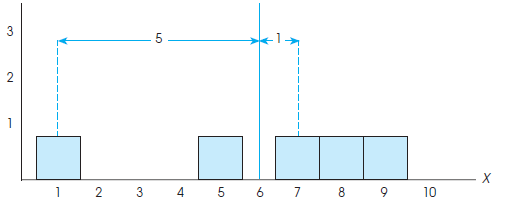
\includegraphics[width = 0.7\textwidth]{./cap1}
	\end{figure}
	\begin{itemize}
		\justifying
		\item Sumar la misma constante a cada valor, NO modifica la desviación estándar.
		\item Multiplicar cada valor por la misma constante, aumenta la desviación estándar en la misma proporción.
	\end{itemize}
\end{frame}

\begin{frame}{¿Por qué dividir sobre $n-1$?}
\begin{itemize}
\justifying
\item Imaginemos una población de N=6 valores: 0,0,3,3,9,9. La media $\mu=4$ y la varianza $\sigma^2=14$.
\item Ahora elegimos muestra de n=2 de esta población.

\begin{center}
\begin{table}[H]
	\scalebox{0.8}{
\begin{tabular}{cccccc} \hline
	\multirow{2}{*}{Muestra} & \multirow{2}{*}{Valor 1} & \multirow{2}{*}{Valor 2} & \multirow{2}{*}{$\bar{X}$} & Varianza & Varianza \\ 
	& & & & Usando $n$ & Usando $n-1$ \\ \hline
1& 0& 0 &0.00 &0.00 &0.00 \\
2& 0& 3 &1.50& 2.25 &4.50 \\
3 &0& 9 &4.50& 20.25& 40.50 \\
4& 3& 0 &1.50 &2.25 &4.50 \\
5& 3& 3 &3.00 &0.00 &0.00 \\
6& 3& 9 &6.00 &9.00 &18.00 \\
7& 9& 0 &4.50 &20.25& 40.50 \\
8& 9& 3 &6.00 &9.00 &18.00 \\
9& 9& 9& 9.00 &0.00& 0.00\\  \hline
& & Totales & 36.00 & 63.00 & 126.00 \\
\end{tabular}}
\end{table}
\end{center}
\end{itemize}
\end{frame}
%%%%%%%%%%%%%%%%%%%%%%%%%%%%%%%%%%%%%
 \section{Valor Z}
\begin{frame}{Valores Z}
\begin{itemize}
\justifying
\item Supongamos que en un examen cualquiera, la nota recibida es $X=76$. ¿Es buena o mala la nota?
\pause \item Si la media es $\mu=70$, sé que estoy 6 puntos por encima de la media.
\pause \item Aún teniendo información de la media, no es posible saber dónde está localizado el valor de la nota.
	\begin{figure}[H]
		\centering  
		\caption{ } 
		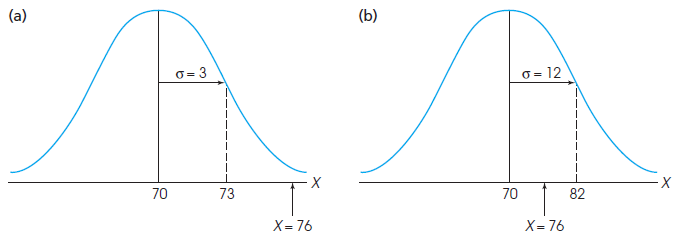
\includegraphics[width = 0.7\textwidth]{./cap2}
	\end{figure}
\end{itemize}

\end{frame}

\begin{frame}
\begin{itemize}
\justifying
\item La ubicación relativa del valor dentro de una distribución depende tanto de la media como de la desviación estándar.
\item Los valores Z tienen dos objetivos:
\begin{enumerate}
	\justifying
\item Reportar la ubicación exacta de un valor dentro de una distribución.
\item Permitir la comparación entre dos distribuciones estandarizadas. 
\end{enumerate}
\item ¿Se puede comparar un puntaje de 64 en la sección de matemáticas de Saber Pro con un puntaje de 66 directamente, si se sabe que cada prueba fue realizada en períodos diferentes?
\item Si la media de ambos exámenes fue 62, además $\sigma_1=1$ y $\sigma_2=4$ ¿A quién le fue mejor?

\end{itemize}
\end{frame}

\begin{frame}
	\begin{center}
	\begin{block}{Valor Z}
		\justifying
		Un valor Z reporta la ubicación precisa de cada valor X dentro de la distribución. Su signo señala si el valor está por encima o por debajo de la media. Además, el valor numérico especifica la distancia de la media al contar el número de desviaciones estándar entre el valor y la media.
	\end{block}
		\end{center}
\begin{itemize}
\justifying
\item La fórmula para calcular el valor Z es la siguiente:
$$Z_X=\dfrac{X-\bar{X}}{s_X}$$
\item La unidad de medida del valor Z son el número de desviaciones estándar (SD).
\end{itemize}
\end{frame}

\begin{frame}
\begin{itemize}
\justifying
\item Volvamos al ejemplo de la prueba Saber Pro.
\item Para el puntaje de 64, donde $\bar{X}=62$ y $\sigma_1=1$:
$$Z_X=\dfrac{64-62}{1}=\dfrac{2}{1}=+2 SD$$
\item Para el puntaje de 66, donde $\bar{X}=62$ y $\sigma_1=4$:
$$Z_X=\dfrac{66-62}{4}=\dfrac{4}{4}=+1 SD$$
\item La fórmula en muchas ocasiones no es necesaria. Si $\bar{X}=10$ y $s_x=2$, cuál es el valor de Z para un X=8?
\end{itemize}

\end{frame}

\begin{frame}
\begin{itemize}
\justifying
\item Al estandarizar una distribución:
\begin{enumerate}
\item su forma se mantiene.
\item La media se convierte en $\mu=0$.
\item La desviación estándar será $\sigma=1$.
\end{enumerate}
	\begin{figure}[H]
		\centering  
		\caption{ } 
		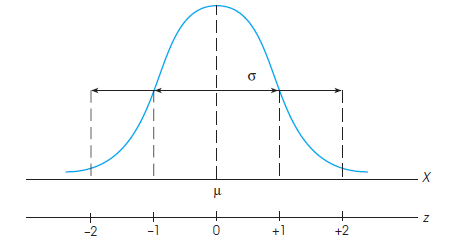
\includegraphics[width = 0.6\textwidth]{./cap3}
	\end{figure}
\end{itemize}
\end{frame}

\begin{frame}{La Regla 68-95-99}
\begin{center}
	\scalebox{0.9}{
\begin{tikzpicture}
\begin{axis}[no markers, domain=0:10, samples=100,
axis lines*=left, xlabel=Desviaciones estándar, ylabel=Frecuencia,,
height=6cm, width=10cm,
xtick={-3, -2, -1, 0, 1, 2, 3}, ytick=\empty,
enlargelimits=false, clip=false, axis on top,
grid = major]
\addplot [fill=cyan!20, draw=none, domain=-3:3] {gauss(0,1)} \closedcycle;
\addplot [fill=orange!20, draw=none, domain=-3:-2] {gauss(0,1)} \closedcycle;
\addplot [fill=orange!20, draw=none, domain=2:3] {gauss(0,1)} \closedcycle;
\addplot [fill=blue!20, draw=none, domain=-2:-1] {gauss(0,1)} \closedcycle;
\addplot [fill=blue!20, draw=none, domain=1:2] {gauss(0,1)} \closedcycle;
\addplot[] coordinates {(-1,0.4) (1,0.4)};
\addplot[] coordinates {(-2,0.3) (2,0.3)};
\addplot[] coordinates {(-3,0.2) (3,0.2)};
\node[coordinate, pin={68.2\%}] at (axis cs: 0, 0.4){};
\node[coordinate, pin={95\%}] at (axis cs: 0, 0.3){};
\node[coordinate, pin={99.7\%}] at (axis cs: 0, 0.2){};
\node[coordinate, pin={34.1\%}] at (axis cs: -0.5, 0){};
\node[coordinate, pin={34.1\%}] at (axis cs: 0.5, 0){};
\node[coordinate, pin={13.6\%}] at (axis cs: 1.5, 0){};
\node[coordinate, pin={13.6\%}] at (axis cs: -1.5, 0){};
\node[coordinate, pin={2.1\%}] at (axis cs: 2.5, 0){};
\node[coordinate, pin={2.1\%}] at (axis cs: -2.5, 0){};
\end{axis}
\end{tikzpicture}}
\end{center}
\end{frame}

\begin{frame}{La Utilidad de la Regla}
\begin{itemize}
\item Imaginemos una muestra de 1000 mujeres de la universidad. Su peso medio es de $\bar{X}=60 kgs$ y su desviación estándar es $s_X=5 kgs$.
\item 500 mujeres tendrán menos de 60 kgs.
\item Cerca de 680 mujeres pesarán entre 55 y 65 kgs.
\item Alrededor de 950 mujeres pesan entre 50 y 70 kgs.
\item Aproximadamente 3 pesarán menos de 45 y más de 75 kgs.
\end{itemize}

\end{frame}


\end{document}